\documentclass[12pt, twocolumn]{amsart}
\usepackage{geometry} % see geometry.pdf on how to lay out the page. There's lots.
\usepackage{epigraph}
\usepackage{graphicx}
\usepackage{url}
\usepackage{wrapfig}
\usepackage[francais]{babel}
\usepackage[utf8]{inputenc} % encodage
\usepackage[T1]{fontenc} % encodage
\geometry{a4paper} % or letter or a5paper or ... etc
% \geometry{landscape} % rotated page geometry
\graphicspath{{illustrations/}}
% See the ``Article customise'' template for come common customisations
\title{Le miroir du cinéma}
\author{Julia Callebat}
% \date{} % delete this line to display the current date
%%% BEGIN DOCUMENT
\begin{document}
\maketitle

\cleardoublepage
\onecolumn
\tableofcontents


\cleardoublepage
\twocolumn
\section*{Introduction}
\vspace*{10mm}
La Pologne, de par son histoire, a longtemps été un pays multiculturel qui a accueilli tout au long de son histoire des peuples d'origines très différentes. Avant la période des partages\footnote{Annexions successives du territoire de la Pologne-Lituanie au XVIIIe siècle (1772, 1793, 1795) par l'Empire de Russie, le Royaume de Prusse et l'Empire d'Autriche.}, le territoire de la Pologne était composé de deux pays distincts : la Couronne - correspondant au Royaume de Pologne - et le Grand Duché de Lituanie où vivaient Lituaniens, futurs Biélorusses et Ukrainiens. Il s'agissait aussi d'une terre d'accueil pour les Juifs fuyant les persécutions d'Europe occidentale. \\
Après le déplacement des frontières en 1945\footnote{Les frontières de la Pologne sont modifiées par les accords de Yalta à la fin de la Seconde Guerre mondiale.}, la Pologne, de pays multiculturel et multilingue, tend à devenir monolithique - une seule langue, une seule religion, une seule origine. Or, la réalité est plus complexe ; c'est uniquement dans une Pologne démocratique que la place aux minorités nationales - à côté d'autres minorités - devient un sujet abordé dans les arts. Il est important par ailleurs de dissocier le point de vue des élites artistiques et intellectuelles de celui d'un milieu plus rural et souvent moins ouvert. Il peut être alors compliqué de comprendre comment ces minorités sont vues par les Polonais et pourquoi elles sont souvent rejetées. Alors pourquoi ne pas se pencher sur un art qui bien souvent, en trame de fond d'une histoire, dépeint avec précision et justesse la réalité de la vie en Pologne pour ces minorités, que ce soit de nos jours ou au siècle dernier : le cinéma ?\\
Le cinéma polonais est souvent méconnu à l'étranger, en partie à cause de ses thèmes qui lui sont propres. Et pourtant, ces thèmes délicats de la co-responsabilité des Polonais dans le massacre des Juifs durant la guerre, du rejet de l'homosexualité par une partie de la population - qui pourtant n'est pas absent, même au sein du clergé, des crimes commis au nom du nationalisme dans les régions dites "retrouvées", imposées à la Pologne après la guerre, ne sont traités véritablement que depuis le XXIe siècle, voire depuis 2010. \\
Je vais donc tenter, par l'analyse de quelques films qui abordent ces sujets épineux et souvent très controversés, de comprendre et de vous faire découvrir quelle est la réalité de la vie en Pologne pour ses minorités. 

\clearpage
\section{Les jeunes}

\paragraph{}
On ne peut pas vraiment parler de minorité en ce qui concerne les jeunes : tout le monde a été jeune un jour, et les jeunes forment une partie importante de la société. Et pourtant, il s’agit d’une partie de la population qui est souvent incomprise, qui connait ses problèmes propres, ses questionnement et ses drames qui sont souvent rejetés par les autres comme n’étant que des enfantillages, et critiqués par ceux qui, ayant grandis, voient le monde bien différemment et peinent à comprendre – voire ne cherchent pas à comprendre la complexité du comportement de jeunes d’aujourd’hui. Même parmi la jeunesse elle-même se créent des groupes qui se rejettent mutuellement, qui se critiquent sans chercher à se comprendre et qui se blessent dans leur recherche propre d’identité et de maturité. Alors quand viennent se mêler aux problèmes inhérents à cet âge adolescent où chacun se cherche, les questions de l’homosexualité, du rapport parfois conflictuel avec Internet et les univers particuliers comme celui du mouvement emo, on se rend compte qu’il existe au sein même de cette jeunesse au traitement particulier des minorités silencieuses, ignorées le plus souvent, sinon critiquées et rejetées.

\subsection*{Sala Samobojcow - La Chambre de Suicidés}\footnote{Scénario et réalisation de Jan Komasa, sorti en 2011}
\paragraph{}
Dominik est un jeune que l’on verrait comme normal : fils d’une riche famille, entourés d’amis, son chemin semble tout tracé – une vie facile, faite d’argent, de fêtes et de plaisirs. Mais lui ne s’y sent pas à son aise, et cherche un sens à sa vie au milieu de toute la superficialité qui l’entoure, tout en suivant le flot de cette vie qui lui a été offerte. Sa vie bascule le jour où, au cours d’une soirée, il embrasse un de ses amis – pour le jeu, pour la fête, un baiser sans autre signification que celle d’une jeunesse qui s’amuse sans limites. Dès le lendemain commence pour lui la dure épreuve de la persécution sur Internet. Ses amis l’accusent d’homosexualité, le rejettent, se moquent de lui et tous ses amis se transforment en bourreaux. Ici apparait, bien que cela ne soit en rien le sujet du film, l’homophobie sous-jacente qui existe dans la jeunesse en général, par rejet de ce qui est différent, mais surtout en Pologne, où l’homosexualité reste un sujet délicat et controversé.


\begin{wrapfigure}[24]{o}{8cm}

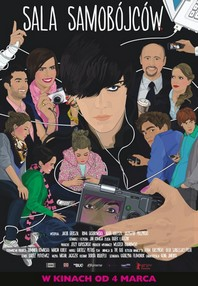
\includegraphics[width=7cm]{sala.jpg}

\end{wrapfigure}
\clearpage
Le problème plus grave qui est soulevé par ce film est la relation conflictuelle que peuvent avoir les jeunes avec Internet, et les dangers que peuvent représenter les réseaux sociaux entre les mains de jeunes qui réagissent à l’étranger par la haine et la violence. Du jour au lendemain, un jeune qui était intégré dans la société, populaire, riche, possédant tout ce que la superficialité adore, se retrouve un paria de la société, un exclus qui se retranche dans sa chambre pour ne plus en sortir, qui se retrouve seul face au reste du monde et qui sombre dans la dépression. Ce problème du cyber harcèlement, relativement récent, est un grand problème de la nouvelle génération qui reste malheureusement trop souvent ignoré et qui peut avoir des conséquences désastreuses. 
Dans sa solitude et sa dépression, avec sa sensibilité d’adolescent qui se cherche, et qui cherche un sens à sa vie qui jusque-là ne semblait en avoir aucun, va se tourner aussi vers Internet pour chercher consolation et réponses. S’ouvre alors à lui la magie des mondes virtuels – magnifiquement représentés dans le film par des séquences en images de synthèse de paysages irréels, froids et pourtant magnifiques. Sur Internet, il découvre alors des communautés qu’il ne connaissait pas, bien loin du monde de superficialités dans lequel il a grandi, et plus particulièrement la communauté emo, ces jeunes qui rejettent la vie et développent une fascination pour l’auto-destruction et la mort. Il y rencontre une jeune fille pour qui il se passionne, et qui, sans jamais qu’ils ne se rencontrent dans la vraie vie, le guide au travers de cette vie virtuelle dans laquelle il sombre, et l’emmène dans la « Chambre des suicidés », un espace de discussion de jeunes suicidaires. Dominik devient alors lui aussi intellectuellement et sensiblement fasciné par la scarification, le suicide et la mort, jusqu’à se perdre complètement. Pendant toute sa période d'enfermement, personne ne viendra le voir, ses quelques relations avec ses anciens amis se dématérialisent complètement et ses parents - homme politique et femme d'affaire - ne trouvent jamais de temps pour lui, au point qu'ils ne se rendent pas compte qu'il n'est pas sorti de sa chambre pendant plusieurs jours. \\
Ce film traite de thèmes qui ne sont pas particuliers à la Pologne, mais qui sont des problèmes de sociétés présent dans bien des pays : les relations qu'ont les jeunes avec Internet, que ce soit à travers la dématérialisation des relations, du cyber-harcèlement, ou des rencontres parfois dangereuses qu'on peut y faire, ainsi que l'adolescence, la recherche de soit dans un monde matériel, dans une famille sans amour ni même présence parentale. Roman Polanski, lors de sa visite à Paris en 2014 pour la première de "Vénus à la fourrure" (2013), a dit que le film de Komasa, s'il n'avait été tourné en polonais par des Polonais, aurait été l'un des plus grands film du cinéma mondial de ces dernières années. Il est passé largement inaperçu en dehors des frontières de la Pologne, non à cause de son sujet mais à cause de la langue et des problèmes de distributions des films des pays de taille moyenne. 
\clearpage
\section{La Mazurie}
\paragraph{}
La notion d'identité nationale est très récente, surtout dans les milieux ruraux où les peuples s'identifiaient au travers de leur langue, de leur religion et de leurs terres. La Mazurie, région aux peuples d'origines très diverses - polonais, allemands, hollandais, français... -, a été rattachée à la Pologne en 1945. Les Mazurs, habitants de cette région, ont vécus une germanisation forcée durant l'entre-deux-guerres, mais se considéraient bien souvent plus polonais qu'allemands. En 1944, avec l'avancée de l'armée rouge, de nombreux Mazurs on fuit devant les atrocités commises par les soviétiques lors de leur passage (pillage, viols, meurtres...). Ceux qui restèrent durent alors faire face à l'animosité des Polonais - souvent colons venus de l'extrême est de la Pologne, nouvellement rallié à l'URSS - qui les voyaient comme Allemands. L'état polonais organisa une politique d'expulsion des Mazurs des territoires nouvellement acquis, anciennement allemands. D'un autre côté, les civils polonais habitant ces régions ont eu une attitude ambiguë, certains se livrant au pillage, au lynchage et au meurtre. En 1955, les Mazurs acquirent le titre de minorité polonaise, et le gouvernement leur accorda des aides économiques. Le comportement des soldats soviétiques durant cette période fut aussi varié, certains maltraitant Polonais et Mazurs indifféremment, d'autres essayant de les protéger.
\subsection*{Roza - Rose}\footnote{Réalisé par Wojciech Smarzowski, sorti en 2011}
\paragraph{}
En 1945, Tadeusz, un ancien officier de l'Armia Krajowa, la principale force de résistance polonaise durant la guerre, dont la femme a été violée et tuée par des soldats Allemands, se rend en Mazurie pour donner à Roza quelques objets personnels de son mari, Mazur enrôlé de force dans la Wehrmacht, qu'il a vu mourir. Elle lui demande alors de rester chez elle, dans sa ferme, pour la protéger des brigands et des violences qu'elle a déjà connu dans cette région où règne l'anarchie après la guerre. Peu à peu, cette relation purement pratique se teinte de respect et d'amour, ce qui est très mal vu par les nouveaux nationalistes polonais et par le NKVD soviétique. Et surtout, Roza étant considérée comme Allemande par le nouveau gouvernement polonais, risque de se faire expulser. \\
\begin{wrapfigure}[24]{o}{8cm}

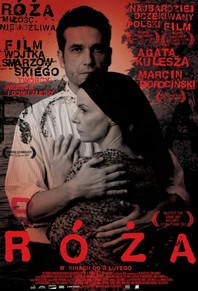
\includegraphics[width=7cm]{roza.jpg}

\end{wrapfigure}
\clearpage
Bien que le thème principal de cette histoire soit l'histoire d'amour qui se crée entre deux personnages détruits par la guerre et les brutalités qui ont suivi, le fond historique dépeint parfaitement les conditions des minorités ethniques de Mazurie durant cette période. Il s'agit d'ailleurs de l'un des très rares films qui osent toucher à cette partie délicate de l'histoire de la Pologne, où de nombreuses atrocités ont été commises au nom du nationalisme. A la fin de l'occupation nazie Roza, veuve, mazure, se retrouve rejetée par la société, dénigrée, et violée à de mutliples reprises par les soviétiques. Des nouveaux habitants de cette région, Polonais, elle ne reçoit que du mépris à cause de ses origines que les Polonais comprennent mal. Car Roza est d'origine polonaise avant tout, bien qu'elle se soit avant la guerre intégrée à la société et à la culture allemande. Génération née avant la Première Guerre mondiale et la politique de nationalisation forcée menée par l'Allemagne, elle parle majoritairement polonais ; sa fille, en revanche, née durant l'entre-deux-guerre, parle presque uniquement allemand mais ne se considère pas pour autant comme Allemande. Leur histoire est celle de beaucoup de ces Mazurs : longtemps considérés - et se considérant souvent eux-mêmes - comme Slaves, ou Polonais, les habitants de cette région ont dû faire face à une nationalisation forcée lorsque les territoires de la Mazurie faisait encore partie de l'Allemagne. Puis, lorsque la Mazurie a été rattachée à la Pologne, une deuxième vague de nationalisation forcée, cette fois polonaise, achève de détruire ce peuple et en fait une minorité rejetée par tous ; origines polonaises, éducation allemande, coutumes slaves, traditions allemandes, noms polonais, prénoms allemands, langue polonaise, écriture allemande, neutralité politique.... Toutes ces caractéristiques de cette minorités engendrent incompréhension et donc rejet de la part de tous, qui la voient comme étrangère. Aujourd'hui, il ne reste presque plus de Mazurs en Pologne : il s'agit d'un peuple exterminé moins par la guerre que par ses conséquences dans un pays totalitaire ne supportant pas l'altérité. Et avec eux ont disparus des coutumes traditionnelles et toute une culture, essentiellement orale, que ce film nous fait découvrir.  
\clearpage
\section{Les homosexuels}
Pays profondément catholique, la Pologne a longtemps rejeté violemment l’homosexualité, comme étant un péché et un crime, un comportement déviant qui doit être réfréné ou soigné. Dans la Pologne Populaire\footnote{Ce terme (PRL en polonais) désigne la période allant de la fin de la guerre aux transformations politiques de 1989.} en revanche le thème des minorités sexuelles est resté un tabou - l'idéologie voulait qu'elles n'existent pas. Ce n'est qu'à la fin des années 90 que l'art commence à briser ce tabou en Pologne. Cependant, face aux tentatives d'affirmation, d'émancipation parfois trop affichées de ces minorités, se développent une réaction de rejet dans une partie de la population. Les médias catholiques polonais véhiculent des messages homophobes et des images très négatives des gay et des lesbiennes.
\begin{figure}

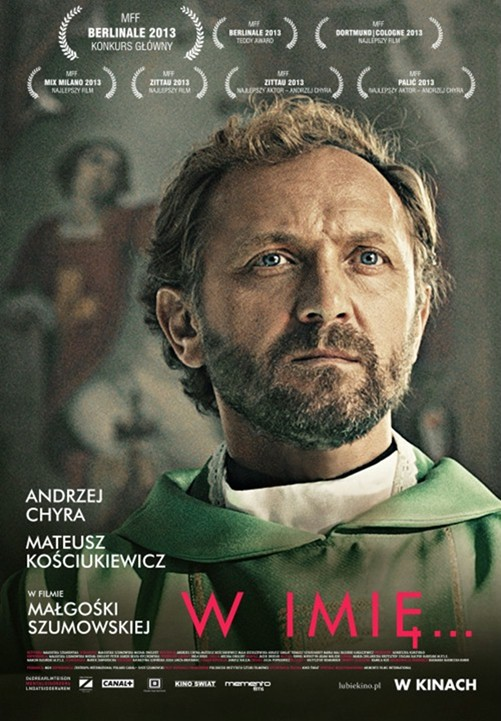
\includegraphics[width=7cm]{wimie.jpg}

\end{figure}


\subsection*{W Imie... - Aime et fais ce que tu veux}\footnote{Réalisé par Malgorzata Szumowska, sorti en 2013}
\paragraph{}
Dans la campagne polonaise, le prêtre Adam, jeune, dynamique et autoritaire, se retrouve en charge d’un centre pour jeunes garçons en difficultés de sa nouvelle paroisse. Avec une démarche assez éloignée du conservatisme religieux qui reste important en Pologne, il prend en main cette jeunesse perdue et violente et s’impose rapidement comme une figure charismatique très respectée dans ce village où il s’est installé. Mais alors qu’il aide ces jeunes à résoudre leurs problèmes par la prière, le travail physique et le sport, il se retrouve confronté à ses propres angoisses et problèmes qui le poursuivent inconsciemment depuis des années : son questionnement constant sur la foi, ses problèmes d’alcoolisme et, surtout, son homosexualité reniée, qu’il tente de fuir et de rejeter, mais qui ne cesse de s’imposer à lui au contact de ces jeunes dont il doit s’occuper. Et lorsqu’il finit par nommer ce secret inconscient, qu’il finit par dire à sa sœur, sa seule confidente (qui vit au Canada) « Je suis une pédale », celle-ci ne le croit pas et le croit juste perdu – alors que, et le film nous le montre bien, ce n’est qu’à partir du moment où il a réussi à accepter son homosexualité qu’Adam cesse d’être perdu.\\
 Mais si Adam finit petit à petit à s’accepter et qu’il se rapproche de l’un des garçons dont il s’occupe – et qui a lui-même développé une fascination plus qu’amicale envers le prêtre -, cela ne passe pas inaperçu aux yeux de l’un de ses seuls amis dans ce village – dont la femme a d’ailleurs, par ennui, tenté en vain de séduire le prêtre- qui s’en va le dénoncer auprès de l’archevêque de la région. Celui-ci lui demande alors la plus grande discrétion, argumentant que « dans l’Eglise, on ne remue pas la poussière sous le tapis » et se charge de changer Adam de paroisse, sans bien sûr nommer de cause à ce changement. Ce passage est une allusion non cachée aux quelques problèmes et scandales que connait l’Eglise, notamment en Pologne, où il existe un malaise profond lié aux non-dits dans les cas d'homosexualité dans le clergé polonais. Il faut savoir aussi qu’en Pologne, dans ce cadre d’homophobie sous-jacente, certains font l’amalgame entre homosexualité et pédophilie. Ce film ne traite cependant pas de ces scandales-là : même s’il s’agit de jeunes garçons, tous ont entre 18 et 25 ans. Pour la réalisatrice, il s’agit, au travers d’un film artistique, d’aborder un sujet qui dérange, de montrer les choses telles qu’elles sont réellement et non telles que les stéréotypes négatifs les décrivent. Il est à noter cependant que, dans cette Pologne à deux vitesses où les milieux ruraux restent fermés et souvent homophobes, les élites intellectuelles et artistiques brisent les tabous depuis le début des années 2000, et que l'homophobie polonaise est en très net déclin.
\\ \\
La preuve en est la très bonne réception de ce film par les critiques, la presse et le public, avec l’exception notable d’un journal de droite chrétien conservateur qui l’a dénoncé comme une œuvre « dégoutante ». \emph{W Imie…} a même été récompensé lors de festivals de cinéma à Berlin et à Gdynia (en Pologne), ce qui, selon la réalisatrice, explique que de nombreux journaux conservateurs ne se soient pas prononcés sur ce film. Et si quelques critiques l’accusent d’avoir joué la carte du prêtre pédophile dans l’unique but de faire polémique et s’attirer les grâces des critiques cinématographiques, plus nombreux sont ceux qui louent le traitement artistique de ce problème de société très présent en Pologne. Cependant cela ne signifie pas du tout que les minorités gay et lesbienne ne sont plus discriminées et sont totalement acceptées par la population. Une des raisons du succès de ce film est la véracité de sa description de l’homosexualité en Pologne. Le prêtre passera plus de la moitié du film à essayer de la combattre, à la refuser, à se questionner, à se considérer comme sale et pêcheur à cause de ses pensées, et l’un des jeunes à sa charge se suicidera à la suite d’une relation homosexuelle avec l’un des autres jeunes du centre. Cette relation peut nous sembler extrême, mais montre bien à quel point est ancrée dans la pensée et dans l’éducation polonaise le dégoût de l’homosexualité - en tout cas en ce qui concerne le milieu rural où se déroule ce film. Ce suicide fait d’ailleurs écho à l’histoire de Dominik dans \emph{Sala Samobojcow} qui, bien que hétérosexuel, se fera rejeter violemment par ses amis au point de tomber dans la dépression. \\
Si des artistes polonais osent aujourd’hui traiter du problème épineux de l’homosexualité en Pologne, et si le public et la presse (mis à part la presse catholique conservatrice) acceptent ces œuvres et les images qu’elles véhiculent, loin des stéréotypes négatifs, le problème n’en reste pas moins entier, et il reste beaucoup à faire encore, au niveau notamment de l’éducation sexuelle des jeunes, afin que non seulement les homosexuels soient acceptés dans la société mais aussi – et surtout – qu’ils commencent par s’accepter eux-mêmes.
\clearpage
\section{Les Juifs}
Si la Pologne est l’un des pays où les juifs ont le plus souffert durant la Seconde Guerre mondiale, c’est principalement parce qu’il s’agissait d’un des pays en Europe où la minorité juive était la plus nombreuse : plus de 15\% avant la guerre, dont 90\%  seront mort d'ici à 1946. Aujourd’hui la minorité juive en Pologne est très faible mais grandissante, notamment par un phénomène singulier mais relativement courant en Pologne : des hommes et des femmes qui, adultes, découvrent leurs origines juives – qu’ils s’agissent d’orphelins n’ayant jamais connus leurs parents, morts durant les massacres, ou d’enfants dont les parents dissimulent toujours leurs origines et pratiquent leur religion en secret. Pourquoi donc un tel phénomène ? Si la Pologne a été historiquement le premier pays à accepter les Juifs sans discrimination, l’antisémitisme croissant depuis le XVIIIe s'intensifie dans les années 1930. Depuis, les Polonais connaissent une relation très conflictuelle avec les populations juives de leur pays. En effet, s’il n’y a pas eu de véritable collaboration entre les Polonais et les nazis, comme il y a pu en avoir sous le régime de Vichy en France, la majorité de la population pendant la guerre restait indifférente aux problèmes des juifs (ghetto, déportation…). Sans parler du pogrom de Jedwabne où entre 300 et 1500 juifs - selon les sources - ont été tués par des paysans polonais, l’antisémitisme des Polonais s’exprimait non par des délations mais, et comme depuis plusieurs décennies, par un rejet été un mépris sous-jacent envers les personnes d'origines juives. De nos jours, si la Pologne n’est plus aussi largement antisémite et que la minorité juive est acceptée sans discrimination, il existe un complexe historique vis-à-vis de la population juive qui en fait un sujet toujours très délicat, même 70 ans plus tard.
\begin{figure}

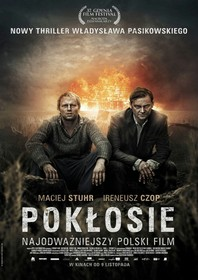
\includegraphics[width=7cm]{poklosie.jpg}

\end{figure}
\subsection*{Poklosie - La glanure}\footnote{Réalisé par Wladyslaw Pasikowski, sorti en 2012}
\paragraph{}
Sous les aspects d’un thriller dramatique, \emph{Poklosie} traite du très controversé massacre de Jedwabne d’un point de vue très actuel. Il suit l’histoire de deux frères, l’un vivant sur les terres de ses parents dans la campagne polonaise et l’autre revenant pour des vacances des Etats-Unis où il a émigré. Tous deux se retrouvent face à face avec ce village rural polonais de Gorowka - version fictive de Jedwabne, où les autochtones les rejettent et cherchent à les faire partir. A force de se défendre et de chercher la vérité derrière ces attaques, les deux hommes découvrent l’horrible vérité : en 1941, les habitants de leur village et des alentours raflent les Juifs, et les tuent publiquement en les faisant brûler dans un entrepôt, avant d’enterrer leurs restes dans un champ et de récupérer leurs terres. \\
Ce massacre, attribué pendant très longtemps aux  Einsatzgruppen, soulève aujourd’hui encore une vive controverse, certains niant encore l’implication des paysans polonais, et les historiens ne parviennent pas à déterminer avec certitude si ce massacre a été dirigé par des soldats allemands ou s’il s’agissait d’une initiative des Polonais. Le film, lui, prend clairement parti et semble affirmer qu’il n’y avait aucune part de responsabilité allemande dans ce massacre. La sortie de ce film a donc violemment ravivé le débat à ce sujet, au point que l’un des acteurs principaux de ce film a affirmé qu’il est plus simple en Pologne aujourd’hui de se dire gay que de se dire juif. En effet, il existe un très fort complexe polonais vis-à-vis des comportements qui ont pu exister durant la guerre, avec un important refus d’accepter les erreurs et les horreurs commises. Comme montré dans le film, les paysans, encore des années après, refusent d’admettre que les terres sur lesquelles ils se trouvent, habitent et travaillent, ont appartenu à une époque à des Juifs. 
\\
Dans les débats enflammés qui ont eu lieu dans la presse et sur Internet à la sortie de ce film, si certains remettent en question la véracité du fond historique, d’autres s’attachent plus à la présentation qu’en fait le film. Certains s’y opposent vivement en critiquant la qualité artistique, et un internaute va jusqu’à dire que « le scénario a été écrit en vertu des exigences de contes de fées pour les jeunes Israéliens ». D’autres au contraire louent la qualité de ce thriller qui approche un sujet très important de l’histoire polonaise qui a encore une place majeure dans l’actualité. Mais plus que tout, ce film – et le fait que cette polémique soit toujours d ‘actualité plus de 70 ans plus tard – montre à quel point la relation des Polonais avec les juifs et avec leur histoire reste conflictuelle et difficile. 

\begin{wrapfigure}[24]{o}{8cm}

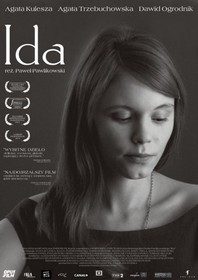
\includegraphics[width=7cm]{ida.jpg}

\end{wrapfigure}
\clearpage
\subsection*{Ida}\footnote{Réalisé par Pawel Pawlikowski, sorti en 2013}
\paragraph{}
En 1962, la jeune Ida, orpheline et pieuse novice, quitte le couvent où elle vit depuis son enfance, pour aller passer quelques jours chez sa tante avant de prononcer ses vœux et devenir nonne, comme le lui conseille sa mère supérieure. Chez sa tante, juge stalinienne devenue alcoolique, elle apprend que ses parents étaient juifs, et qu'ils ont disparus durant l’occupation nazie. Elle décide alors de partir avec sa tante dans le village où ses parents ont vécu, afin de savoir ce qui leur est vraiment arrivé. Mais sur place règne la loi du silence, et nul n’avoue avoir connu sa famille. \\
Cette loi du silence que l'on retrouve dans ce film comme dans \emph{Poklosie} est très représentative de l'état de la Pologne après guerre, pendant plusieurs décennies. De nos jours, nombreux sont ceux qui cherchent la vérité sur les événements des années de guerre, mais toujours existe cette réaction de silence et de dissimulation ; face à la lourde histoire des Juifs de Pologne durant la Seconde Guerre mondiale, dans ce profond traumatisme de la population polonaise, si certains se tournent vers un devoir de mémoire et de vérité, d'autres préfèrent se voiler la face et refusent d'accepter les crimes qui ont été commis - non pas qu'ils aient forcément une responsabilité directe dans ces atrocités commises envers les Juifs, mais cette culpabilité latente d'avoir été un peuple fortement antisémite et d'avoir, sinon aidé, du moins laissé les nazis massacrer les Juifs, pèse lourdement sur la conscience collective polonaise, ce qui explique à la fois cette volonté de taire les événements et de nier les massacres mais aussi ce désir de faire éclater la vérité pour enfin accepter les horreurs du passé.\\
Un des éléments narratif les plus marquant de ce film est la découverte par cette jeune novice, pieuse chrétienne prête à vouer sa vie à l'Eglise, de ses origines juives. Il ne s'agit de loin pas d'un cas isolé ou d'une fantaisie du réalisateur. Après la guerre, dans les années 1960-70, nombreux sont ceux qui ont découvert leurs origines juives ; par exemple, un prêtre très connu, Jakub Weksler Waszkinel, a appris à 33 ans qu'il était juif, à la mort de ses parents adoptifs. Il s'agit généralement de Polonais nés juste avant ou pendant la Seconde Guerre Mondiale, et qui ont été cachés depuis leur enfance dans des institutions religieuses afin d'être protégés contre les nazis. \\

Récompensé et nominé de nombreuses fois, \emph{Ida} a été accueilli très chaleureusement par les critiques et le public, que ce soit pour la beauté de sa mise en scène (en noir et blanc, format 16/9 tout comme les films des années 1960) qui nous plonge au coeur de cette Pologne de 1962, ou que soit pour la profondeur de ses caractères et de cette intrigue somme toute assez banale dans la Pologne de l'après guerre, et pourtant si étonnante pour ceux qui ne savent pas. Certains ont cependant reproché à Pawlikowski de concevoir un film trop "symétrique" où la distribution des "fautes" entre les Polonais et les Juifs est trop parfaite (l'antisémitisme et les crimes contre les Juifs d'une part, les atrocités staliniennes, dues à ce qu'on appelle "zydokomuna" (les communistes juifs d'après-guerre), de l'autre. C'est dire à quel point la problématique des relations polono-juives reste épidermique encore dans la Pologne d'aujourd'hui. 

\cleartoevenpage

\section*{Le mot de la fin}
\vspace*{10mm}
\paragraph*{}
Les différents films présentés dans ce dossier font partie du mouvement artistique et intellectuel présent en Pologne depuis le début du XXIe siècle, qui cherche à briser les tabous de l'époque communiste. Cependant ce mouvement reste lent - \emph{Roza} est le premier film à traiter de la problématique des minorités de Mazurie après la guerre, et les films sur la thématique des Juifs de Pologne restent très rares. Si en France il existe des - mauvais et souvent inconnus - films comiques sur la Shoah, en Pologne, un film tel que \emph{Poklosie} déclenche une vague de débats enflammés. De même, un film mettant en scène des homosexuels en France ne suscitent pas des polémiques comme l'a fait \emph{W Imie...}. La question juive reste par ailleurs beaucoup plus délicate en Pologne, notamment car les Polonais ont assisté de près aux massacres des Juifs - ghettos, camps de concentration sur le territoire polonais - sans parler du nombre de morts polonais ou sur le sol polonais à cause de la guerre. Si certains artistes cherchent à choquer par la violence et l'extrémisme de leurs prises de position, comme c'est le cas dans \emph{Poklosie} où le réalisateur mélange différents faits historiques pour construire un concentré de violence faites par des Polonais sur des Polonais - juifs ou non -, d'autres cherchent la conciliation, montrant à égalité les torts des Polonais et des Juifs qui occuperont souvent des positions hauts placées dans le pouvoir et la juridiction de la Pologne communiste - alors que les torts ne sont absolument pas symétriques - comme dans \emph{Ida}.

Pour ce qui est des autres minorités ethniques polonaises - Mazurs, Tziganes... - le sujet reste moins brûlant car la responsabilité est bien plus souvent du côté des dirigeants qui ont mené des politiques d'expulsion et d'exclusion sociale que du côté de la population. Cependant, bien qu'il s'agisse de thèmes moins délicats, ils n'en restent pas moins très peu abordés. La question du traitement des Tziganes en Pologne durant le siècle dernier n'a été que très récemment évoqué pour la première fois dans un film, \emph{Papusza} (2013) de Krzysztof Krauze. 

\clearpage
\onecolumn
\begin{thebibliography}{100}

\bibitem{SS}
	Jan Komasa,
	\emph{La Chambre des Suicidés},
	(\emph{Sala Samobojcow}),
	2011.
	
\bibitem{R}
	Wojciech Smarowski,
	\emph{Rose},
	(\emph{Roza}),
	2011.
	
\bibitem{WI}
	Malgorzata Szumowska,
	\emph{Aime et fais ce que tu veux},
	(\emph{W Imie...}),
	2013.
	
\bibitem{P}
	Wladyslaw Pasikowski,
	\emph{La glanure},
	(\emph{Poklosie}),
	2012.
	
\bibitem{I}
	Pawel Pawlikowski,
	\emph{Ida},
	2013.

\bibitem{HKP}
	Tadeusz Lubelski, 
	\emph{Historia kina polskiego. Tworcy, filmy, konteksty},
	Videograf II,
	Chorzow,
	2009.
	 
\bibitem{OWK}
	Barbara Hollender,
	\emph{Od Wajdy do Komasy},
	Proszynski i S-ka,
	Varsovie,
	2014.
	
\bibitem{RP}
	Małkowska Monika and Świątek Rafał,
	\emph{W sieci i w realu},
	mai 2014,
	url=http://www.rp.pl/artykul/620631.html.

\bibitem{wiki:salaSamobojcow}
	Wikipedia,
	\emph{Sala Samobojcow},
	mars 2014,
	url=http://pl.wikipedia.org/wiki/Sala\_samobójców.


\bibitem{PISF}
	Różdżyńska Aleksandra,
	\emph{Komasy filmy o dojrzewaniu},
	janvier 2010,
	url=http://www.pisf.pl/pl/kinematografia/news/komasy-filmy-o-bezkompromisowym-dojrzewaniu.


\bibitem{AI}
	Lakomski Marcin,
	\emph{Être homosexuel(le) en Pologne},
	février 2012,
	url=http://www.amnesty.be/doc/s-informer/notre-magazine-le-fil/libertes-archives/les-anciens-numeros/381-Numero-de-Fevrier-2002/Dossier,81/article/etre-homosexuel-le-en-pologne.

\bibitem{CI}
	Ostapkowicz Iwona,
	\emph{"Aime et fais ce que tu veux" : un film qui brise les tabous},
	décembre 2013,
	url=http://www.courrierinternational.com/article/2013/12/18/aime-et-fais-ce-que-tu-veux-un-film-qui-brise-les-tabous-0.

\bibitem{wiki:wImie}
	Wikipedia,
	\emph{"W Imie..."},
	décembre 2013,
	url=http://pl.wikipedia.org/wiki/W\_imię...

\bibitem{GPL}
	Michałek Mateusz,
	\emph{Recenzja filmu "W imię..."},
	janvier 2014,
	url=http://www.film.gildia.pl/filmy/w-imie/recenzja.

\bibitem{WPL}
	Felis Paweł,
	\emph{"W imię..." - film o bezczelności pożądania od dziś w kinach},
	septembre 2013,
	url=http://wyborcza.pl/1,75475,14637890,\_W\_imie\_\_\_\_\_\_\_film\_o\_bezczelnosci\_pozadania\_od\_dzis.html.


\bibitem{CZPR}
	Szumowska Małgorzata,
	\emph{Małgorzata Szumowska: "W imię..." to nie jest kontrowersyjny film},
	septembre 2013,
	url=http://www.polskieradio.pl/10/2940/Artykul/937647,Malgorzata-Szumowska-W-imie-to-nie-jest-kontrowersyjny-film.

\bibitem{wiki:histoireDesJuifsEnPologne}
	Wikipedia,
	\emph{Histoire des Juifs en Pologne},
	novembre 2014,
	url=http://fr.wikipedia.org/wiki/Histoire\_des\_Juifs\_en\_Pologne.


\bibitem{wiki:massacreJedwabne}
	Wikipedia,
	\emph{Massacre de Jedwabne},
	septembre 2014,
	url=http://fr.wikipedia.org/wiki/Massacre\_de\_Jedwabne.

\bibitem{LMDR}
	Papin Alice,
	\emph{De nombreux Polonais ignoraient qu'ils étaient Juifs},
	février 2014,
	url=http://www.lemondedesreligions.fr/savoir.

\bibitem{wiki:poklosie}
	Wikipedia,
	\emph{Poklosie},
	janvier 2015,
	url=http://pl.wikipedia.org/wiki/Pokłosie.

\bibitem{FWP}
	Walkiewicz Michał,
	\emph{Pokłosie},
	février 2012,
	url=http://www.filmweb.pl/film/Pok\%C5\%82osie-2012-624892.

\bibitem{NTD}
	Redakcja Natemat,
	\emph{Dlaczego "Pokłosie" Władysława Pasikowskiego wywołało prawdziwą medialną burzę?},
	février 2012,
	url=http://natemat.pl/39235,dlaczego-poklosie-wladyslawa-pasikowskiego-wywolalo-prawdziwa-medialna-burze-waszym-zdaniem.

\bibitem{NTL}
	Majdan Krzysztof,
	\emph{Łatwiej powiedzieć: "Jestem gejem" niż "Jestem Żydem" - to nie zaściankowość tylko historyczny kompleks},
	février 2012,
	url=http://natemat.pl/39141,latwiej-powiedziec-jestem-gejem-niz-jestem-zydem-to-nie-zasciankowosc-tylko-historyczny-kompleks.

\bibitem{FWI}
	Walkiewicz Michał,
	\emph{Ida},
	septembre 2013,
	url=http://www.filmweb.pl/film/Ida-2013-546529.

\bibitem{LI}
	Icher Bruno,
	\emph{Ida, nonne stop},
	février 2014,
	url=http://next.liberation.fr/cinema/2014/02/11/ida-nonne-stop\_979510.

\bibitem{wiki:ida}
	Wikipedia,
	\emph{Ida},
	janvier 2015,
	url=http://fr.wikipedia.org/wiki/Ida\_(film).

\bibitem{wiki:mazurie}
	Wikipedia,
	\emph{Mazurie},
	octobre 2014,
	url=http://fr.wikipedia.org/wiki/Mazurie.

\bibitem{wiki:expulsionAllemandsEuropeEst}
	Wikipedia,
	\emph{Expulsion des Allemands d'Europe de l'Est},
	janvier 2015,
	url=http://fr.wikipedia.org/wiki/Expulsion\_des\_Allemands\_d'Europe\_de\_l'Est.

\bibitem{FWR}
	Grochowska Malwina,
	\emph{Roza},
	octobre 2011,
	url=http://www.filmweb.pl/film/R\%C3\%B3\%C5\%BCa-2011-564694.

\bibitem{wiki:roza=}
	Wikipedia,
	\emph{Roza},
	juin 2014,
	url=http://en.wikipedia.org/wiki/Rose\_(2011\_film).

\bibitem{SK}
	AZ,
	\emph{Sukcesy "Róży" nie ustają - jest Grand Prix we Francji},
	octobre 2013,
	url=http://stopklatka.pl/wiadomosci/-/75803552,sukcesy-rozy-nie-ustaja-jest-grand-prix-we-francji.

\bibitem{CPL}
	Zarębski Konrad,
	\emph{Wojciech Smarzowski - Rose - Interview},
	décembre 2014,
	url=http://culture.pl/en/article/wojciech-smarzowski-rose-interview.

\end{thebibliography}

\end{document}